\subsection{Défintion}

\begin{mydef}
	Un parallélogramme est un quadrilatère dont les \kw{côtés opposés sont parallèles}.
\end{mydef}

\begin{myex}
	%\begin{multicols}{2}
		
		
		\begin{center}
			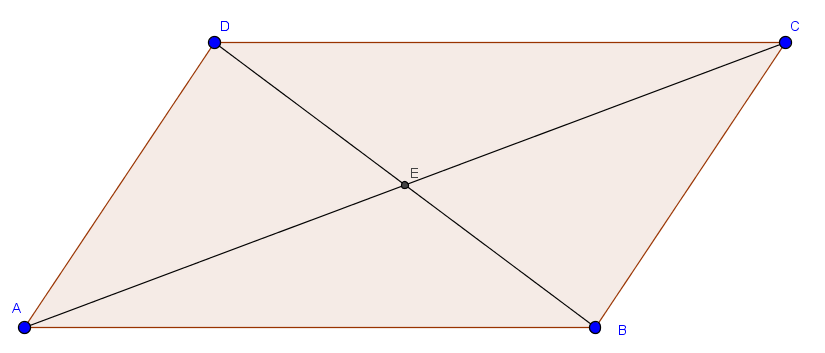
\includegraphics[scale=0.15]{para}
		\end{center}
	
	On a $(AB) // (CD)$ et $(BC) // (AD)$ donc le quadrilatère ABCD est un parallélogramme.
	%\end{multicols}
\end{myex}

\subsection{Propriétés du parallélogramme}

	\begin{myprops}
		Si un quadrilatère est un parallélogramme alors :
		\begin{itemize}
			\item ses \kw{côtés opposés} sont \kw{parallèles} deux à deux;
			\item ses \kw{côtés opposés} ont la \kw{même longueur};
			\item ses \kw{diagonales se coupent en leur milieu};
			\item ses \kw{angles opposés} sont \kw{égaux} deux à deux;
			\item \kw{deux angles successifs} sont \kw{supplémentaires};
			\item le point d'intersection de ses diagonales est son \kw{centre de symétrie}.
		\end{itemize}
	
		
	\end{myprops}


	\begin{myex}
		\begin{multicols}{2}
			Dans le parallélogramme ABCD :
			\begin{itemize}
				\item $(AB)$ // $(CD)$ et $(AD) // (BC)$;
				\item $AD = BC$ et $AB = CD$;
				\item $AO = OC$ et $BO = OD$;
				\item $\widehat{BAD} = \widehat{DCB}$ et $\widehat{ADC} = \widehat{CBA}$;
				\item $\widehat{BAD} + \widehat{ADC} = 180\degree$  et \\ $\widehat{DCB} + \widehat{CBA} = 180$\degree;
				\item $O$ est le centre de symétrie.
			\end{itemize}
			
			
			
			\begin{center}
				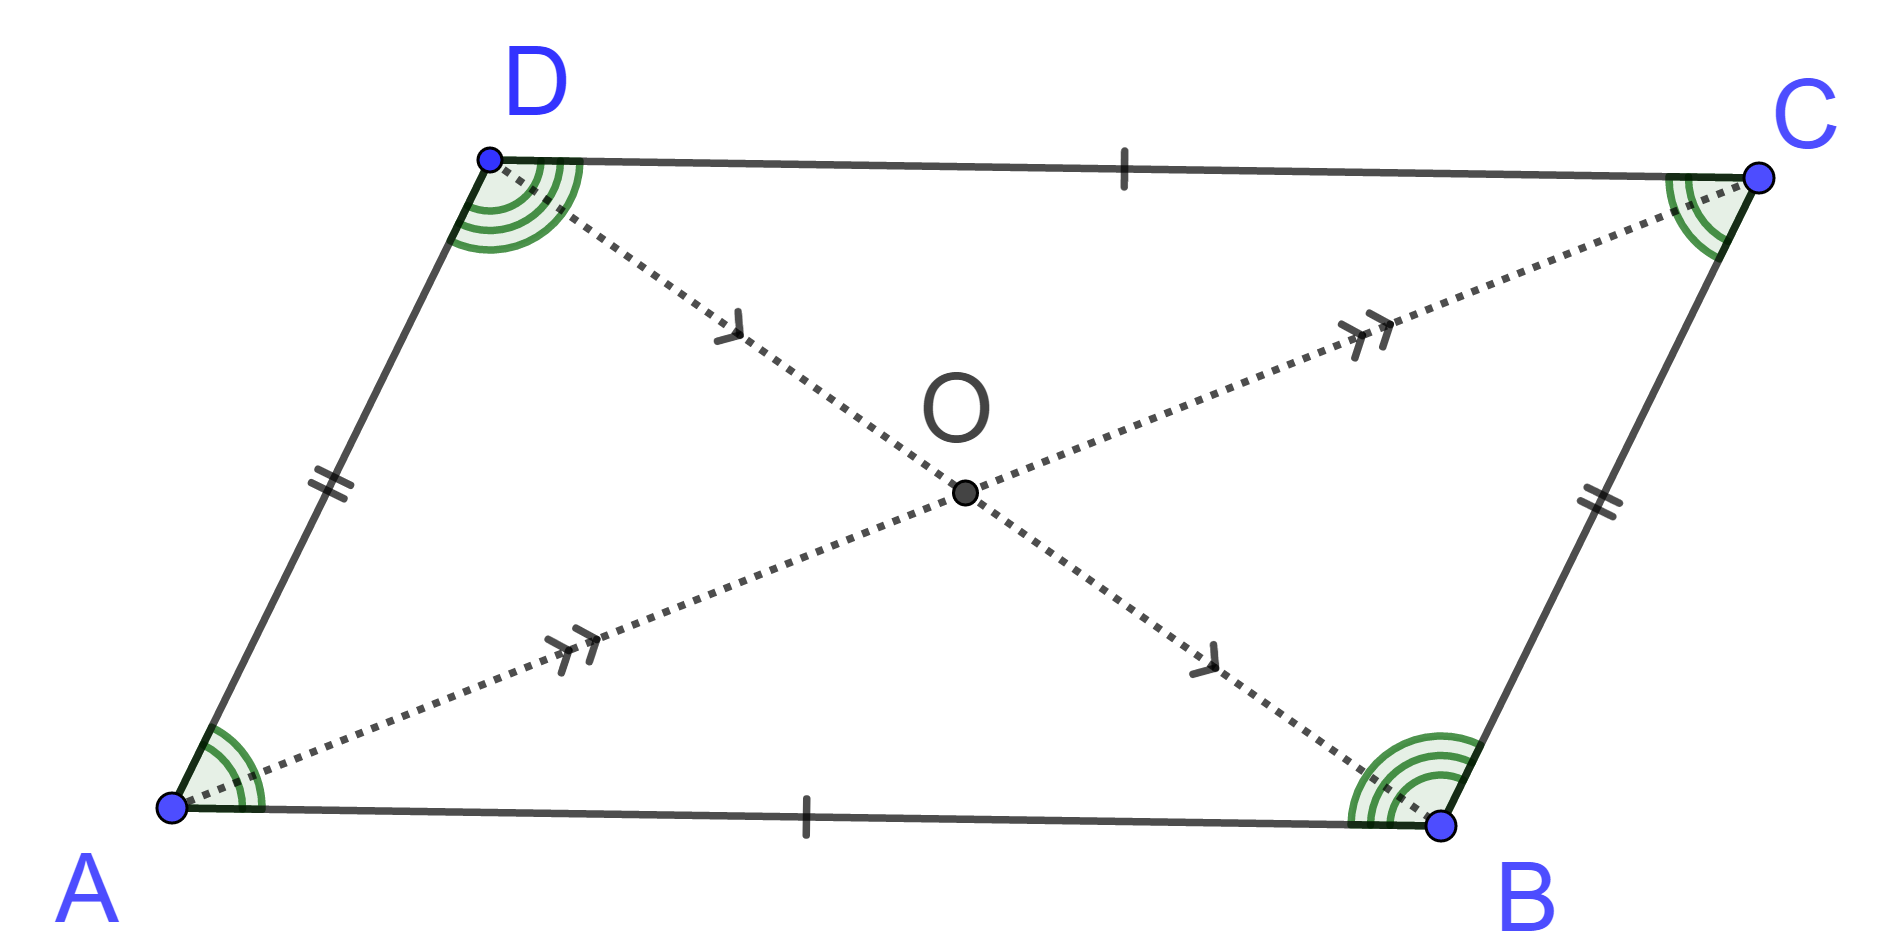
\includegraphics[scale=0.17]{para2}
			\end{center}
		\end{multicols}
	\end{myex}